\documentclass{article}
% Teacher-supplied style is copied byte-for-byte; preprint shows the named authors.
\usepackage[preprint,nonatbib]{neurips_2021}
\usepackage[utf8]{inputenc}
\usepackage[T1]{fontenc}
\usepackage[authoryear,round]{natbib}
\usepackage{hyperref,url,booktabs,amsfonts,microtype,xcolor,graphicx,tabularx,array,capt-of}
\urlstyle{same}
\setlength{\bibhang}{0.5in}
\setlength{\bibsep}{0pt}
\renewcommand{\bibsection}{\begin{center}\normalsize\bfseries References\end{center}}
\hypersetup{hidelinks,pdftitle={Credit Card Default Prediction},pdfauthor={SC6122 Group 5}}
% Course metadata only: do not imply submission to or acceptance by NeurIPS.
\makeatletter
\renewcommand{\@noticestring}{NTU SC6122 Emerging Topics in FinTech --- Group 5 course project.}
\makeatother
\title{Credit Card Default Prediction:\\Ranking Risk and Choosing an Action}
\author{ \textbf{Lei Peng} (G2509090C) \quad \textbf{Zhang Hanyu} (G2509091L) \\ \textbf{Zhou Xinzhe} (G2509033F) \quad \textbf{Xu Yiqun} (G2509092H) \\ Nanyang Technological University \\ SC6122 Emerging Topics in FinTech --- Group 5 }
\begin{document}
\maketitle
\thispagestyle{plain}
\begin{abstract}
We compare logistic regression, a decision tree, random forest and XGBoost on 30,000 historical credit-card clients. Shared fitting, validation and test partitions separate hyperparameter selection from threshold choice. Tree regularization improves the decision-tree baseline; selected RF and XGBoost have similar test average precision. XGBoost tuning does not improve test ranking, but a validation-selected threshold reduces hypothetical cost by 7.52\% under a 5:1 missed-default-to-false-alarm cost ratio. The policy flags 55.72\% of clients, exposing a substantial review burden. The results distinguish predictive ranking from action policy and support further validation with realistic costs and capacity limits, rather than immediate deployment.
\end{abstract}
\section{Problem, objectives and data}
Credit default prediction can prioritize account reviews, but missed defaults and unnecessary reviews have different consequences. We ask: \textbf{how well can models identify default risk, and how should ranking ability, interpretability and decision cost be balanced?} We compare logistic regression (LR), a decision tree (DT), random forest (RF) and XGBoost using average precision (AP), ROC-AUC, predictive explanations and hypothetical error costs.

We use UCI's Default of Credit Card Clients dataset \citep{uci}: 30,000 Taiwan clients, 23 predictors and a binary outcome (1 = default). Predictors cover credit limit, demographics, repayment status, bills and payments during April--September 2005; amounts are in NT dollars. There are 6,636 defaults (22.12\%). An always-negative classifier therefore appears accurate while detecting no defaults. The dataset also underlies a published comparison of default-prediction methods \citep{yeh}.

\textbf{Cleaning and identity.} No entries are missing. EDUCATION 0/5/6 are mapped to 4 (345 rows), and MARRIAGE 0 to 3 (54 rows). Other values are retained, including negative repayment codes and amounts. No rows are removed: 35 identical feature--label repetitions remain, and 15 test feature vectors also occur in development. This potential dependence is acknowledged without altering the established split after evaluation.

The transformation reproduces the committed clean data in values, types and order. The newly downloaded UCI source and its hash are archived; original download bytes were not retained. The zero-based \texttt{row\_id} is UCI ID minus one; neither identifier enters the models.
\newpage
\section{Experimental design and model selection}
\begin{center}
\begin{minipage}{\linewidth}
\captionof{table}{Fixed stratified partitions (seed 42). Inner CV uses 14,400 fitting and 3,600 holdout rows per fold.}
\label{tab:split}\centering
\begin{tabularx}{\linewidth}{@{}lrX@{}}\toprule
Partition & Clients & Purpose\\\midrule
Fitting & 18,000 & Five-fold CV; final fitting with selected parameters\\
Validation & 6,000 & Selection of decision thresholds\\
Test & 6,000 & Evaluation of frozen models and decisions\\\bottomrule
\end{tabularx}
\end{minipage}
\end{center}
The 24,000 development rows are stratified into 18,000 fitting and 6,000 validation rows; 6,000 test rows remain separate (seed 42). Positive counts are 3982, 1,327 and 1,327. All four reported runs use identical development memberships and five CV folds. Final models fit only the 18,000 fitting rows, with no later validation refit.

Preprocessing uses scikit-learn pipelines \citep{sklearn}, fitted within each CV training fold. SEX, EDUCATION and MARRIAGE are one-hot encoded with unknown categories ignored. LR additionally learns numeric StandardScaler statistics within the fold. Tree models retain numeric scales. No missing-value imputation or sampling is used. Selected class weights are part of the training configuration, not a change to test prevalence. Pipelines prevent categories or scaling moments from being learned on validation/test data.

\textbf{Hyperparameters.} The common selection objective is mean five-fold AP. Equal scores prefer the lowest candidate index. DT uses exhaustive grid search; RF/XGBoost evaluate a specified baseline plus 23 seeded random candidates. LR evaluates 12 exhaustive settings. These are comparable splits and objectives, not identical computational budgets.
\begin{center}
\begin{minipage}{\linewidth}
\captionof{table}{Declared search budgets and selected configurations. Complete settings and per-fold scores accompany the frozen protocols.}
\centering
\begin{tabular}{@{}lrrp{47mm}r@{}}\toprule
Model & Configs & CV fits & Selected (summary) & CV AP\\\midrule
LR & 12 & 60 & C=0.1; unweighted & 0.5113\\
DT & 21 & 105 & Unlimited depth; leaf=100 & 0.5307\\
RF & 24 & 120 & 500 trees; depth=8; leaf=2; class 1:3 & 0.5647\\
XGB & 24 & 120 & 150 trees; depth=4; rate=.03; weight=3 & 0.5620\\
\bottomrule\end{tabular}
\end{minipage}
\end{center}

LR uses L2 logistic regression \citep{esl}, solved with \texttt{lbfgs} (maximum 3,000 iterations); its grid crosses $C$ values .001, .01, .1, 1, 10 and 100 with no class weighting or balanced weighting. DT searches maximum depth 2, 3, 4, 5, 6, 8 or unlimited, and minimum leaf size 1, 20 or 100. RF averages randomized trees \citep{rf}; its search varies tree count, depth, split/leaf size, feature subsampling and class weighting. XGBoost varies tree count, learning rate, depth, child weight, row/column sampling, L1/L2 penalties and positive-class weighting \citep{xgboost}. Baseline tree/ensemble configurations are retained alongside selected configurations.

\textbf{Decision selection.} We use $\hat y=1[s\geq t]$ throughout, where $s$ is the positive-class score. The fixed reference is $t=0.5$. For LR, RF and XGBoost, all distinct validation score cutoffs are considered for $C_r=FP+r\,FN$, with $r\in\{1,3,5,10\}$. Equal costs prefer the largest threshold (fewer alerts); tied scores move together. DT has only its historical fixed 0.5 policy. Each cost threshold is chosen on validation, then applied unchanged to test predictions. No test threshold sweep is used to select a policy.

\textbf{Evaluation scope.} This report compares the recorded model configurations and saved predictions under common evaluation rules. Model and threshold choices were frozen before their final test evaluation. The project test sample had already been examined in earlier work, however, so this retrospective comparison does not constitute fresh independent validation. No further optimization is based on the displayed test results.
\newpage
\section{Ranking and classification findings}
\begin{center}
\begin{minipage}{\linewidth}
\captionof{table}{Test performance at threshold 0.5 ($n=6,000$; default positive). P/R/F1/Acc are proportions; B = baseline, T = CV-selected. Experimental scope is described in Section 2.}
\centering
\begin{tabular}{@{}lrrrrrr@{}}\toprule
Model & AP & ROC-AUC & P & R & F1 & Acc\\\midrule
LR B & 0.4970 & 0.7111 & 0.6975 & 0.2555 & 0.3740 & 0.8108\\
LR T & 0.4967 & 0.7107 & 0.6985 & 0.2532 & 0.3717 & 0.8107\\
DT B & 0.2843 & 0.6076 & 0.3783 & 0.4039 & 0.3907 & 0.7213\\
DT T & 0.5221 & 0.7538 & 0.6583 & 0.3572 & 0.4631 & 0.8168\\
RF B & 0.5312 & 0.7534 & 0.6441 & 0.3806 & 0.4784 & 0.8165\\
RF T & 0.5508 & 0.7752 & 0.5463 & 0.5200 & 0.5328 & 0.7983\\
XGB B & 0.5544 & 0.7773 & 0.6565 & 0.3557 & 0.4614 & 0.8163\\
XGB T & 0.5516 & 0.7762 & 0.5134 & 0.5486 & 0.5304 & 0.7852\\
\bottomrule\end{tabular}
\end{minipage}
\end{center}

\begin{center}
\begin{minipage}{\linewidth}
\captionof{table}{Test confusion counts at 0.5, recomputed from row-aligned scores and labels. B = baseline; T = CV-selected.}
\centering
\begin{tabular}{@{}lrrrrrrrr@{}}\toprule
Model & B: TN & FP & FN & TP & T: TN & FP & FN & TP\\\midrule
LR & 4526 & 147 & 988 & 339 & 4528 & 145 & 991 & 336\\
DT & 3792 & 881 & 791 & 536 & 4427 & 246 & 853 & 474\\
RF & 4394 & 279 & 822 & 505 & 4100 & 573 & 637 & 690\\
XGB & 4426 & 247 & 855 & 472 & 3983 & 690 & 599 & 728\\
\bottomrule\end{tabular}
\end{minipage}
\end{center}

AP is computed by \texttt{average\_precision\_score}, a recall-increment weighted sum of precision, not trapezoidal PR-AUC \citep{ap}. ROC-AUC summarizes positive--negative score ordering. Both use continuous scores and are independent of the chosen operating threshold; precision, recall, F1 and accuracy describe a particular decision rule.
\begin{center}
\begin{minipage}{\linewidth}
\centering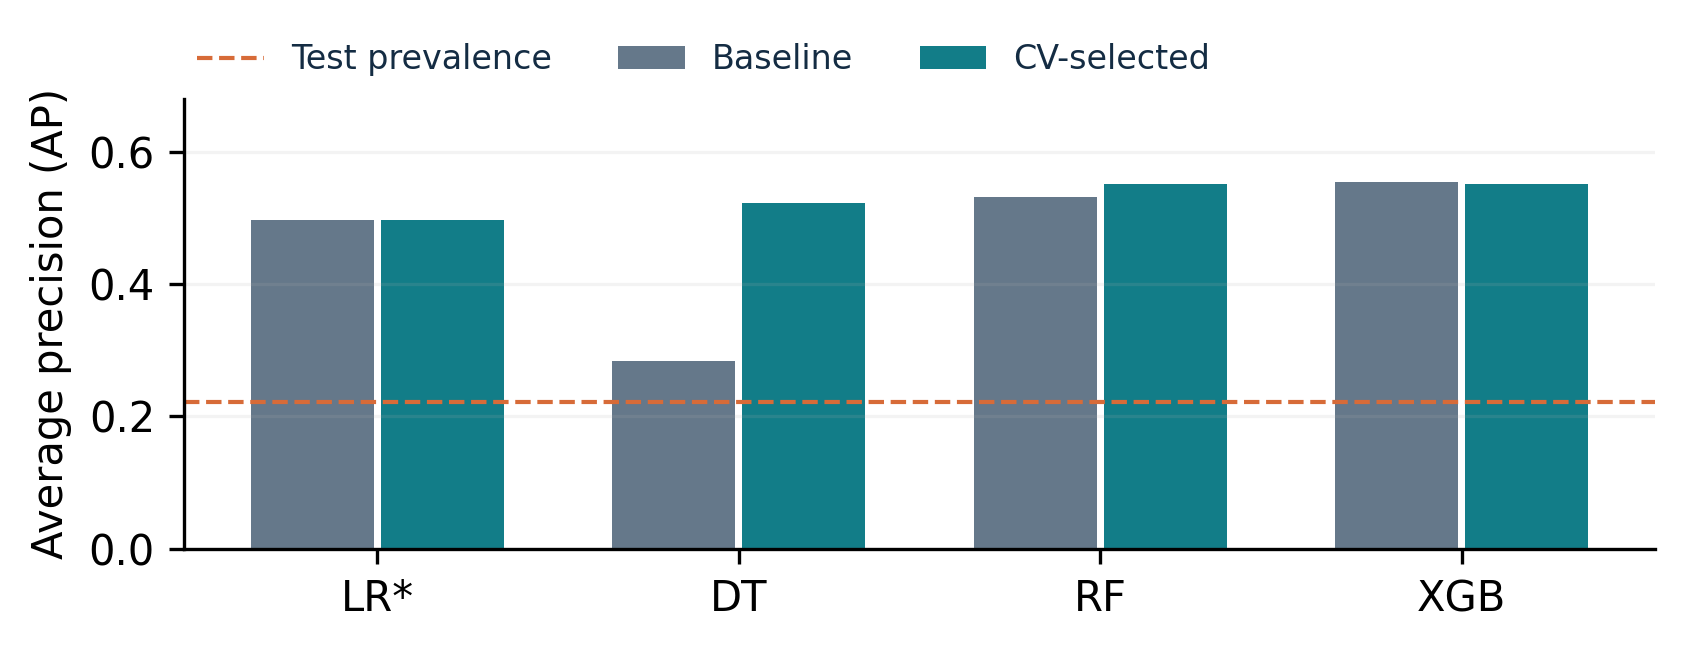
\includegraphics[width=\linewidth]{figures/ranking.png}
\captionof{figure}{Test AP for declared baselines and CV-selected models. The dashed reference is positive prevalence (0.2212). Selection uses fit-fold CV, never this chart.}
\end{minipage}
\end{center}

The unrestricted DT strongly overfits: mean fit-fold AP is about 1.0000 while CV AP is 0.2970. A minimum leaf size of 100 raises test AP from 0.2843 to 0.5221. RF selection raises AP from 0.5312 to 0.5508. XGBoost changes from 0.5544 to 0.5516: the selected configuration does not improve test ranking. LR changes from 0.4970 to 0.4967, also without a ranking gain. Among the displayed point estimates the XGBoost baseline has the highest AP, but this retrospective observation does not authorize a new model-selection round. Small differences between RF and XGBoost do not establish superiority.
\newpage
\section{Thresholds, costs and review capacity}
We treat one false-positive review as one hypothetical cost unit, and a missed default as $r$ units. This is a sensitivity analysis, not a measured monetary loss: loan exposure, loss given default, treatment effects and review capacity are unavailable. Positive class weights can change score calibration, so a probability-derived cutoff such as $1/(1+r)$ is not assumed valid. Policies are selected empirically on validation data.
\begin{center}
\begin{minipage}{\linewidth}
\captionof{table}{Same-model test comparison at 0.5 and the validation-selected $r=5$ policy. Alerts and recall are percentages; cost is FP + 5 FN across 6,000 clients. DT has no historical validation-selected cost policy.}
\centering
\begin{tabular}{@{}lrrrrrrr@{}}\toprule
Model & Policy & Threshold & Recall \% & Alert \% & FP & FN & Cost\\\midrule
LR & 0.5 & 0.50000 & 25.32 & 8.02 & 145 & 991 & 5100\\
LR & Val r=5 & 0.23432 & 59.38 & 32.75 & 1177 & 539 & 3872\\
RF & 0.5 & 0.50000 & 52.00 & 21.05 & 573 & 637 & 3758\\
RF & Val r=5 & 0.32288 & 77.09 & 48.45 & 1884 & 304 & 3404\\
XGB & 0.5 & 0.50000 & 54.86 & 23.63 & 690 & 599 & 3685\\
XGB & Val r=5 & 0.31502 & 82.52 & 55.72 & 2248 & 232 & 3408\\
\bottomrule\end{tabular}
\end{minipage}
\end{center}
\begin{center}
\begin{minipage}{\linewidth}
\centering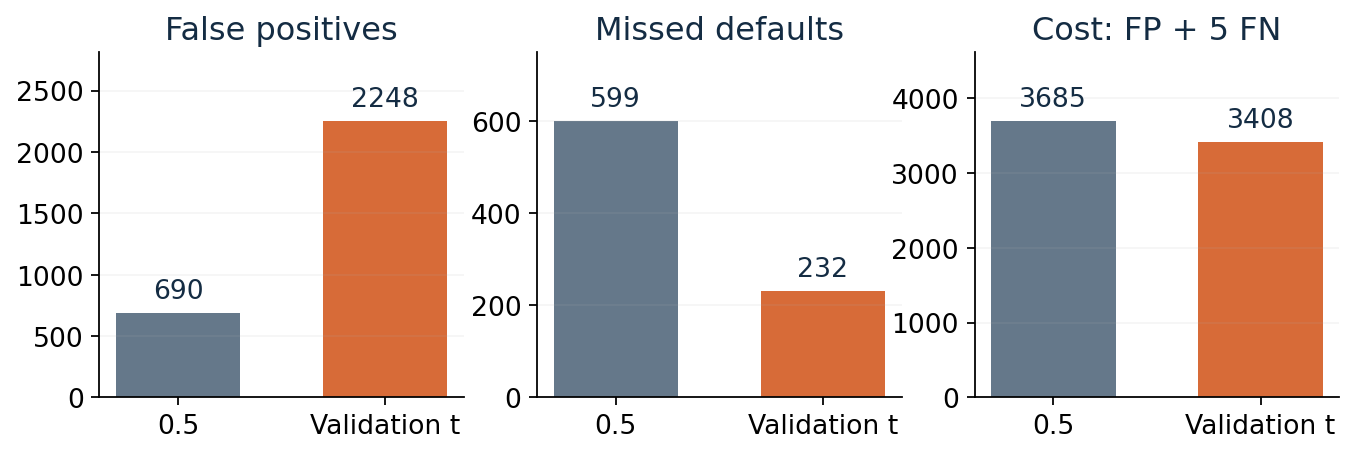
\includegraphics[width=\linewidth]{figures/cost_tradeoff.png}
\captionof{figure}{Moving the same tuned XGBoost from 0.5 to its validation cutoff changes FP/FN and workload. Ranking scores remain unchanged.}
\end{minipage}
\end{center}

For XGBoost, $t=0.31502$ changes cost from 3,685 to 3,408, a reduction of 7.52\%. Recall rises from 54.86\% to 82.52\%, while false positives rise from 690 to 2,248 and 55.72\% of clients are flagged. Precision falls from 51.34\% to 32.76\%. The benefit is fewer missed defaults under the assumed cost ratio; it is not a gain in AP or ROC-AUC. If that review load is infeasible, the policy would need a separately validated capacity constraint, not a threshold changed after viewing test errors.

RF at its validation $r=5$ threshold costs 3,404 and flags 48.45\%, versus XGBoost's 3,408 and 55.72\%. The four-unit difference is too small to support a strong cross-model cost claim. RF detects fewer defaults (77.09\% recall) with fewer false positives. An always-negative policy costs 6,635 and an always-positive policy 4,673 at $r=5$; both are useful context, not deployment recommendations.

\textbf{Uncertainty.} Historical 1,000-replicate stratified paired bootstraps condition on the frozen models, thresholds and fixed class counts. XGBoost's tuned-minus-baseline AP difference is $-0.0028$ (95\% interval $[-0.0106,0.0054]$). The selected-minus-0.5 cost difference is $-46.17$ units per 1,000 (95\% interval $[-74.34,-18.00]$). These intervals describe resampling of fixed predictions; they exclude retraining, hyperparameter/threshold selection, prevalence shifts and new-population uncertainty. They cannot be read as end-to-end deployment guarantees.
\newpage
\section{Interpretation and audit evidence}
\textbf{Complementary explanations.} LR coefficients summarize regularized associations on standardized numeric and encoded categorical scales. Correlated bill/payment variables and full one-hot coding limit isolated coefficient interpretations. DT offers explicit paths: its root splits on \texttt{PAY\_0 <= 1.5}; within fit rows, default proportions are 16.51\% on the left and 70.13\% on the right. These are node-level sample summaries, not causal effects or calibrated individual probabilities. The selected tree has 134 leaves and depth 18: no explicit depth cap does not mean no regularization, since every leaf requires at least 100 observations.

RF averages many trees, making full decision paths less concise. Its saved validation permutation importance identifies recent repayment status, PAY\_0, as most influential: shuffling it reduces AP by 0.1971 on average, versus 0.0196 for PAY\_2. Correlated variables can substitute for one another, and shuffling can create unrealistic combinations; importance describes predictive reliance, not causality. XGBoost instead builds regularized trees sequentially; its threshold trade-offs are evaluated in Section 4.
\begin{center}
\begin{minipage}{\linewidth}
\centering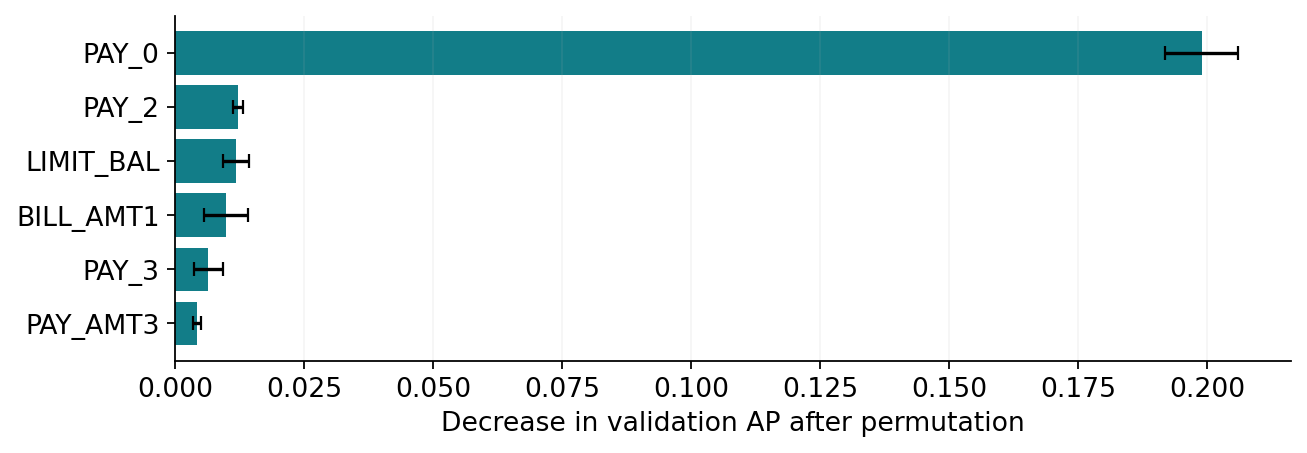
\includegraphics[width=\linewidth]{figures/importance.png}
\captionof{figure}{Tuned random-forest validation permutation importance, top six features. Error bars are the SD across five permutations, not confidence intervals or causal estimates. Horizontal units: decrease in validation AP.}
\end{minipage}
\end{center}

\textbf{Illustrative RF errors.} At 0.5, the selected forest has 637 false negatives and 573 false positives. In the existing saved error export, row 982 defaults despite score 0.1012 and PAY\_0=-2; row 28747 does not default despite score 0.9415 and PAY\_0=3. These most-confident errors illustrate that repayment history is not deterministic; they are not representative average clients and are not used to retune the model. Both threshold-specific case exports satisfy their own classification rules. Extreme cases can remain errors under both policies even when overall error counts change.

\textbf{Reconciliation.} All metrics in the final comparison are recalculated after one-to-one \texttt{row\_id} alignment with actual labels. CSV scores and thresholds use round-trip float parsing. Threshold-equality cases are explicitly tested with $\geq$; no rounding is performed before decisions. Source-train/test hash differences in historical protocols are explained by LF/CRLF serialization, while parsed content, types and order agree. Development and CV membership files are identical across the reproducible models.

Saved models reproduce stored decisions. XGBoost probability replay on this platform differs by at most $5.96\times10^{-8}$ (float32-scale drift) while frozen policy decisions agree; original probabilities remain the reporting source. Model hashes and run metadata are checked, with newline-aware evidence for textual artifacts in the \href{https://github.com/IcantFind-a-username/-SC6122-Group5-Credit-Default}{project repository}. The archived scripts, models and prediction files support result tracing and verification.
\newpage
\section{Conclusions, limitations and contributions}
The models reveal a trade-off: a regularized tree provides inspectable rules, while RF and XGBoost have similar selected-model AP; LR supplies a linear reference. \textbf{Ranking and action policy answer different questions.} XGBoost tuning does not improve test ranking, but its validation-selected threshold reduces hypothetical cost by accepting more false positives. Operational policy must account for costs and review capacity.

Limitations include a single historical population, random rather than temporal/external evaluation, repeated feature vectors, historical test exposure, unequal search budgets and unvalidated calibration. Subgroup errors and fairness have not been assessed; demographic inputs warrant scrutiny. Hypothetical costs omit exposure, realized losses and intervention benefits. Fixed-prediction intervals exclude model-selection uncertainty. Predictive associations do not establish causality, regulatory compliance or production readiness.

Future work should freeze a new protocol on temporal/external data, assess calibration and subgroup errors, and evaluate realistic costs subject to review capacity.

\section*{Member contribution statement}
\begin{center}
\begin{minipage}{\linewidth}
\captionof{table}{Member responsibilities and equal contribution shares.}
\centering
\begin{tabularx}{\linewidth}{@{}p{30mm}Xr@{}}\toprule
Member / student ID & Responsibility and presentation & Share\\\midrule
\shortstack[l]{Lei Peng\\
G2509090C} & Part 1: Data inspection/preprocessing; LR baseline and data characteristics; slides 1--3 & 25\%\\
\shortstack[l]{Zhang Hanyu\\
G2509091L} & Part 2: Decision-tree tuning, learned rules and overfitting control; slides 4--6 & 25\%\\
\shortstack[l]{Zhou Xinzhe\\
G2509033F} & Part 3: Random-forest tuning, feature importance and error cases; slides 7--9 & 25\%\\
\shortstack[l]{Xu Yiqun\\
G2509092H} & Part 4: XGBoost tuning and threshold trade-offs between missed defaults and false alarms; slides 10--12 & 25\%\\
\bottomrule\end{tabularx}
\end{minipage}
\end{center}
Shared responsibilities cover the data split, preprocessing and metrics, integration of the four sections, result checking and presentation preparation.

\section*{AI disclosure}
Generative AI supported language polishing and grammar guidance, together with selected technical tasks. The group retains responsibility for the methods, results, interpretation and acknowledgement of sources.

\newpage
% APA 7 references: alphabetical order, author-date citations, 0.5-inch
% hanging indent, double-spaced entries, sentence-case titles and DOI URLs.
{\normalsize\raggedright\setlength{\baselineskip}{20pt}
\begin{thebibliography}{9}
\bibitem[Breiman(2001)]{rf} Breiman, L. (2001). Random forests. \emph{Machine Learning, 45}(1), 5--32. \url{https://doi.org/10.1023/A:1010933404324}
\bibitem[Chen \& Guestrin(2016)]{xgboost} Chen, T., \& Guestrin, C. (2016). XGBoost: A scalable tree boosting system. In \emph{Proceedings of the 22nd ACM SIGKDD international conference on knowledge discovery and data mining} (pp.\ 785--794). Association for Computing Machinery. \url{https://doi.org/10.1145/2939672.2939785}
\bibitem[Hastie et~al.(2009)]{esl} Hastie, T., Tibshirani, R., \& Friedman, J. (2009). \emph{The elements of statistical learning: Data mining, inference, and prediction} (2nd ed.). Springer. \url{https://doi.org/10.1007/978-0-387-84858-7}
\bibitem[Pedregosa et~al.(2011)]{sklearn} Pedregosa, F., Varoquaux, G., Gramfort, A., Michel, V., Thirion, B., Grisel, O., Blondel, M., Prettenhofer, P., Weiss, R., Dubourg, V., Vanderplas, J., Passos, A., Cournapeau, D., Brucher, M., Perrot, M., \& Duchesnay, \mbox{\'E.} (2011). Scikit-learn: Machine learning in Python. \emph{Journal of Machine Learning Research, 12}(85), 2825--2830. \url{https://jmlr.org/papers/v12/pedregosa11a.html}
\bibitem[scikit-learn developers(n.d.)]{ap} scikit-learn developers. (n.d.). \emph{average\_precision\_score} [API documentation, version 1.8]. \url{https://scikit-learn.org/1.8/modules/generated/sklearn.metrics.average_precision_score.html}
\bibitem[Yeh(2009)]{uci} Yeh, I.-C. (2009). \emph{Default of credit card clients} [Data set]. UCI Machine Learning Repository. \url{https://doi.org/10.24432/C55S3H}
\bibitem[Yeh \& Lien(2009)]{yeh} Yeh, I.-C., \& Lien, C.-H. (2009). The comparisons of data mining techniques for the predictive accuracy of probability of default of credit card clients. \emph{Expert Systems with Applications, 36}(2), 2473--2480. \url{https://doi.org/10.1016/j.eswa.2007.12.020}
\end{thebibliography}}
\end{document}
